%%%%%%%%%%%%%%%%%%%%%%%%%%%%%%%%%%%%%%%%%
%
% CMPT 435
% Fall 2022
% Assignment 1
%
%%%%%%%%%%%%%%%%%%%%%%%%%%%%%%%%%%%%%%%%%

%%%%%%%%%%%%%%%%%%%%%%%%%%%%%%%%%%%%%%%%%
% Short Sectioned Assignment
% LaTeX Template
% Version 1.0 (5/5/12)
%
% This template has been downloaded from: http://www.LaTeXTemplates.com
% Original author: % Frits Wenneker (http://www.howtotex.com)
% License: CC BY-NC-SA 3.0 (http://creativecommons.org/licenses/by-nc-sa/3.0/)
% Modified by Alan G. Labouseur  - alan@labouseur.com
%
%%%%%%%%%%%%%%%%%%%%%%%%%%%%%%%%%%%%%%%%%

%----------------------------------------------------------------------------------------
%	PACKAGES AND OTHER DOCUMENT CONFIGURATIONS
%----------------------------------------------------------------------------------------

\documentclass[letterpaper, 10pt,DIV=13]{scrartcl} 

\usepackage[T1]{fontenc} % Use 8-bit encoding that has 256 glyphs
\usepackage[english]{babel} % English language/hyphenation
\usepackage{amsmath,amsfonts,amsthm,xfrac} % Math packages
\usepackage{sectsty} % Allows customizing section commands
\usepackage{graphicx}
\usepackage[lined,linesnumbered,commentsnumbered]{algorithm2e}
\usepackage{listings}
\usepackage{parskip}
\usepackage{lastpage}
\usepackage{color}

\allsectionsfont{\normalfont\scshape} % Make all section titles in default font and small caps.

\usepackage{fancyhdr} % Custom headers and footers
\pagestyle{fancyplain} % Makes all pages in the document conform to the custom headers and footers

\fancyhead{} % No page header - if you want one, create it in the same way as the footers below
\fancyfoot[L]{} % Empty left footer
\fancyfoot[C]{} % Empty center footer
\fancyfoot[R]{page \thepage\ of \pageref{LastPage}} % Page numbering for right footer

\renewcommand{\headrulewidth}{0pt} % Remove header underlines
\renewcommand{\footrulewidth}{0pt} % Remove footer underlines
\setlength{\headheight}{13.6pt} % Customize the height of the header

\numberwithin{equation}{section} % Number equations within sections (i.e. 1.1, 1.2, 2.1, 2.2 instead of 1, 2, 3, 4)
\numberwithin{figure}{section} % Number figures within sections (i.e. 1.1, 1.2, 2.1, 2.2 instead of 1, 2, 3, 4)
\numberwithin{table}{section} % Number tables within sections (i.e. 1.1, 1.2, 2.1, 2.2 instead of 1, 2, 3, 4)

\setlength\parindent{0pt} % Removes all indentation from paragraphs.

\binoppenalty=3000
\relpenalty=3000

%----------------------------------------------------------------------------------------
%	TITLE SECTION
%----------------------------------------------------------------------------------------

\newcommand{\horrule}[1]{\rule{\linewidth}{#1}} % Create horizontal rule command with 1 argument of height

\title{	
   \normalfont \normalsize 
   \textsc{CMPT 435 - Fall 2022 - Dr. Labouseur} \\[10pt] % Header stuff.
   \horrule{0.5pt} \\[0.25cm] 	% Top horizontal rule
   \huge Assignment One  \\     	    % Assignment title
   \horrule{0.5pt} \\[0.25cm] 	% Bottom horizontal rule
}

\author{Josh Seligman \\ \normalsize joshua.seligman1@marist.edu}

\date{\normalsize\today} 	% Today's date.

\begin{document}
\maketitle % Print the title

\section{Singly Linked List}\label{linkedListSection}
\subsection{The Data Structure}\label{linkedListDataStructure}
A singly linked list is comprised of nodes which contain some form of data as well as a pointer to the next element within the list. As shown in Figure \ref{figure:linkedList}, the final node has a next of \textbf{null}, which marks the end of the list.

\begin{figure}[ht] 
    \centering 
    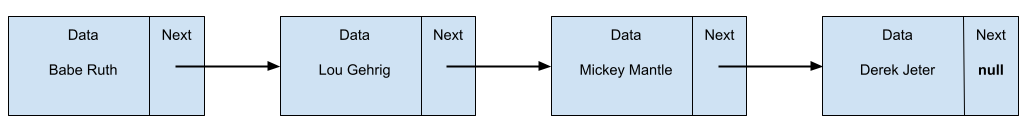
\includegraphics[width=15cm]{linkedList}
    \caption{Example singly linked list of 4 Yankees legends.}
    \label{figure:linkedList}
 \end{figure}

\subsection{Asymptotic Analysis}
Assuming one only has a pointer to the first element in the list, doing any sort of work with the data requires one to start at the beginning and traverse through the list by using the next pointers within each node until the desired operation is complete. For example, as done in Listing \ref{lst:maincpp} within Section \ref{mainProgramListing} on lines 22-26, the only way to dynamically obtain the data for each node was to start at the beginning and iterate through each node by taking advantage of the links. Overall, since linked list operations, such as searching, adding, and removing, all function at a rate of a magnitude of the size of the list, their runtime is classified as $O(n)$.

\subsection{Benefits of a Singly Linked List}
\subsubsection{Limited Size Restrictions}
As previously mentioned in Section \ref{linkedListDataStructure}, the last node within a linked list has a next of \textbf{null}. This characteristic enables linked lists to have no size restrictions barring memory capacity. As a result, this feature makes linked lists preferred over arrays, which have a fixed length, when the size of the data is frequently changing and has an unkown maximum. For instance, as demonstrated in Listing \ref{lst:maincpp} of Section \ref{mainProgramListing} on lines 13-19, the size of the linked list is only limited by our needs and, if needed, more nodes are able to easily be added to the list with their creation as done on lines 13-15 and linking as shown on lines 18 and 19. On the other hand, if the list was made with an array, the size of the array would have to be provided at the time of creation, and it would not be easy to change the size if additional data have to be added to the array.

\subsubsection{Data Type Flexibility}\label{linkedListDataType}
Linked lists do not have to be restricted to be able to store a specific data type. Instead, with the use of generics (C++ templates), the definition of a node is independent of the data type that the user wants to store within the linked list. This provides flexibilty and reusability for many use cases. As demonstrated in Section \ref{nodeListing} Listing \ref{lst:nodeh}, the definition of a node uses a generic T as the type of data being stored, which prevents any assumptions of the data and ensures compatibility with all data types. However, due to how the C++ linker works and to prevent all the code from being written within a single header file, the allowed types have to be stated on lines 13 and 14 in Listing \ref{lst:nodecpp}. This is a C++ specific issue and is not present in other languages such as Java. Regardless, although they have to be specified for C++, any data type can still be stored within a node and a linked list. A demonstration of the user defining which data type is stored in a node is in Section \ref{mainProgramListing} on lines 13-15 of Listing \ref{lst:maincpp}. Instead of the Node class defining the data type, the user is able to specify the type of data they want to store, which is a string in this situation but can be anything they want.

\section{Stack}
\subsection{The Data Structure}\label{stackDataStructure}
A stack uses a last in, first out (LIFO) approach to storing data. The most common analogy for stacks is a stack of plates. Each plate is
placed on top of each other to build the stack when being stored, but the plate on top is always the first to be used. In other words, the most recently plate
that was put away is also the first plate that is taken out. As displayed in Figure \ref{figure:stack}, the stack has a variable called top, which points to the first item in the stack.
Additionally, as shown by the arrows between each element, linked lists are used in the implementation of stacks. Stacks have 3 primary functions: push, pop, and isEmpty.
Push adds a new element to the top of the stack, pop removes the top item from the stack and returns the data, and isEmpty returns whether or not the stack is empty.

\begin{figure}[ht] 
    \centering 
    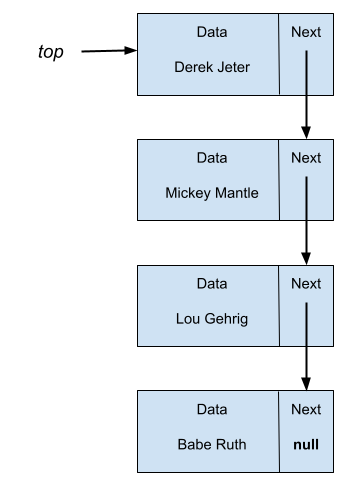
\includegraphics[height=8cm]{stack}
    \caption{Example stack of 4 Yankees legends.}
    \label{figure:stack}
 \end{figure}

\subsection{Benefits of a Stack}
\subsubsection{Time of Individual Data Access}
Stacks are incredibly fast when it comes to the implementation of the push and pop methods. As demonstrated in \textit{stack.cpp} in Section \ref{stackListing},
the push method on lines 21-28 creates the new node for the stack (line 24), points its next element to the current top of the stack (line 26), and then update the top of the stack to
point to the newly created node (line 28). These 3 steps will always run and do not depend on the current size of the stack, which means that the push method runs in $O(1)$ time.
The pop method on lines 30-46 is very similar in that it also executes the same few steps regardless of the current size of the stack. These steps are check if the stack is empty for safety (lines 33-36),
grab the data from the top of the stack (line 39), update the top pointer to point to the second item in the stack (line 40), and return the data (line 44). There is no need to traverse the list because the push
method made the new node the first element of the list, which is equivalent to the top of the stack. Therefore, just like the push method, the pop method also runs in $O(1)$ time.

\subsubsection{Compatibility with the Node Class}
As mentioned in Section \ref{stackDataStructure} and illustrated in Figure \ref{figure:stack}, the stack is implemented using a singly linked list. Therefore, the Stack
class in the code has to utilize the Node class written for singly linked lists, which can be found in Section \ref{nodeListing} and was analyzed in Section \ref{linkedListSection}.
In Section \ref{stackListing}, line 9 in \textit{stack.h} shows that the Stack class has an instance variable that points to the node on the top of the stack. Since the Node
class supports any data type (see Section \ref{linkedListDataType}), the Stack class has to be able to provide a data type for each node to store. For the same reasons as
described in Section \ref{linkedListDataType}, the Stack class also utilizes C++ templates to allow the user to decide which data type gets stored within the stack.
The Stack class is then able to take the data type that the user requests, such as \textbf{char} on line 32 of \textit{main.cpp} in Section \ref{mainProgramListing},
and pass it down to the data type that is stored within each node. This concept is demonstrated in Section \ref{stackListing} in \textit{stack.cpp} on 
line 24 when a new node is created and on line 9 of \textit{stack.h} when defining the top variable for the stack.

\section{Queue}
\subsection{The Data Structure}
A queue uses a first in, first out (FIFO) approach to handling data. One analogy to understand how a queue works is a line to buy movie tickets. The first person that
is in line for these tickets is the first to be assisted at the ticket counter. On the other hand, the last person to enter the line will also be the last one to
buy their ticket. Similar to stacks, queues are implemented using a singly linked list. As displayed in Figure \ref{figure:queue}, queues have a head variable 
that points to the first node within the linked list, which equates to the front of the line for the movie tickets. Queues have 3 primary functions: enqueue, dequeue,
and isEmpty. Enqueue adds a new element to the end of the queue, dequeue removes and returns the first element in the queue, and isEmpty checks to see if the queue is empty or not.

\begin{figure}[ht] 
    \centering 
    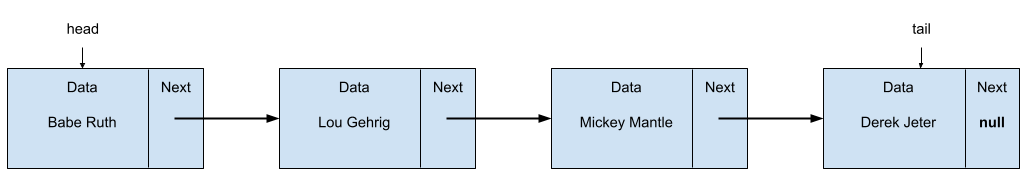
\includegraphics[width=15cm]{queue}
    \caption{Example queue of 4 Yankees legends.}
    \label{figure:queue}
 \end{figure}

\subsection{Benefits of a Queue}
\subsubsection{Compatibility with the Node Class}\label{queueNodes}
The Queue class, just like the Stack class, was implemented using templates to be able to support the use of the Node class, which requires an input of a data type upon
creation. As described in Section \ref{linkedListDataType}, C++ templates enable flexibilty and support for many different data types. Additionally, it is also very
safe to use because creating a Queue (or a Stack or Node) of a given type will result in a data structure that only accepts that type in the future. For instance, if a Queue is created
to support strings, one cannot attempt to enqueue an integer as there will be a type mismatch and the code will not compile. For instance, line 74 of \textit{main.cpp}
in Section \ref{mainProgramListing} is commented out because the compiler cannot convert a string to a single character, which causes a compilation error as the queue
cannot support the string.

\subsubsection{Error Safety}
In addition the the type safety of the templates as described in Section \ref{queueNodes}, the Queue class also has an error measure to prevent users from breaking
the program by doing something that is not allowed. In the case of the Queue class, the error safety occurs if the user tries to dequeue from an empty queue. As displayed on
lines 43-45 of \textit{queue.cpp} in Section \ref{queueListing}, the function checks if the queue is empty and throws an error if it is. This is really important
as, without the check, there would be a runtime error that crashes the program from attempting to work with a null pointer. In the test program for the queue in \textit{main.cpp} of
Section \ref{mainProgramListing}, lines 67-72 use a try-catch block to make sure the programmed error is thrown when attempting to dequeue from an
empty queue. It is of importance to note that this feature is also implemented in the Stack class when attempting to pop from an empty stack (see lines 
33-35 of \textit{stack.cpp} in Section \ref{stackListing}).

\section{Main Program}
\subsection{Program Overview}
The objective of the main program was to print out all the palindromes, ignoring whitespace and capitalization, within a file. More specifically, after normalizing
a string for whitespace and capitalization, each character of the string should be both pushed onto a stack and enqueued on a queue. The stack will hold the
characters in reverse order and the queue will hold each character in the order as they are in the string. Thus, checking to see if the string is a palindrome requires
one to just pop the first character from the stack and dequeue the first character in the queue. If there is ever a time where the characters are different, then
the string is not a palindrome. On the other hand, if every comparison is successful, then the string is a palindrome.


\subsection{Good Parts of the Program}
\subsubsection{File Operations and Output}

\subsubsection{Time Complexity of isPalindrome}


\section{Appendix}
\lstset{numbers=left, numberstyle=\tiny, stepnumber=1, numbersep=5pt}

% Colors and lstset for syntax highlighting from https://www.overleaf.com/latex/examples/syntax-highlighting-in-latex-with-the-listings-package/jxnppmxxvsvk
\definecolor{mygreen}{rgb}{0,0.6,0}
\definecolor{mygray}{rgb}{0.5,0.5,0.5}
\definecolor{mymauve}{rgb}{0.58,0,0.82}
\lstset{
  backgroundcolor=\color{white},   % choose the background color
  basicstyle=\footnotesize,        % size of fonts used for the code
  breaklines=true,                 % automatic line breaking only at whitespace
  captionpos=b,                    % sets the caption-position to bottom
  commentstyle=\color{mygreen},    % comment style
  escapeinside={\%*}{*)},          % if you want to add LaTeX within your code
  keywordstyle=\color{blue},       % keyword style
  stringstyle=\color{mymauve},     % string literal style
}

\subsection{Singly Linked List}\label{nodeListing}
\lstinputlisting[caption=node.cpp, label=lst:nodecpp, language=C++]{./../node.cpp}
\lstinputlisting[caption=node.h, label=lst:nodeh, language=C++]{./../node.h}

\subsection{Stack}\label{stackListing}
\lstinputlisting[caption=stack.cpp, label=lst:stackcpp, language=C++]{./../stack.cpp}
\lstinputlisting[caption=stack.h, label=lst:stackh, language=C++]{./../stack.h}

\subsection{Queue}\label{queueListing}
\lstinputlisting[caption=queue.cpp, label=lst:queuecpp, language=C++]{./../queue.cpp}
\lstinputlisting[caption=queue.h, label=lst:queueh, language=C++]{./../queue.h}

\subsection{Main Program}\label{mainProgramListing}
\lstinputlisting[caption=main.cpp, label=lst:maincpp, language=C++]{./../main.cpp}

\end{document}